\chapter{Prototype design}

In order to effectively assess the effectiveness of a clustering model we created a prototype interface that could be used to demo the different features when usability testing. We created a web application called ProvOwl that reads provenance from the PROV format and renders a directed acyclic graph that users can explore by panning, zooming and rearranging nodes.

\begin{figure}[h]
\centering
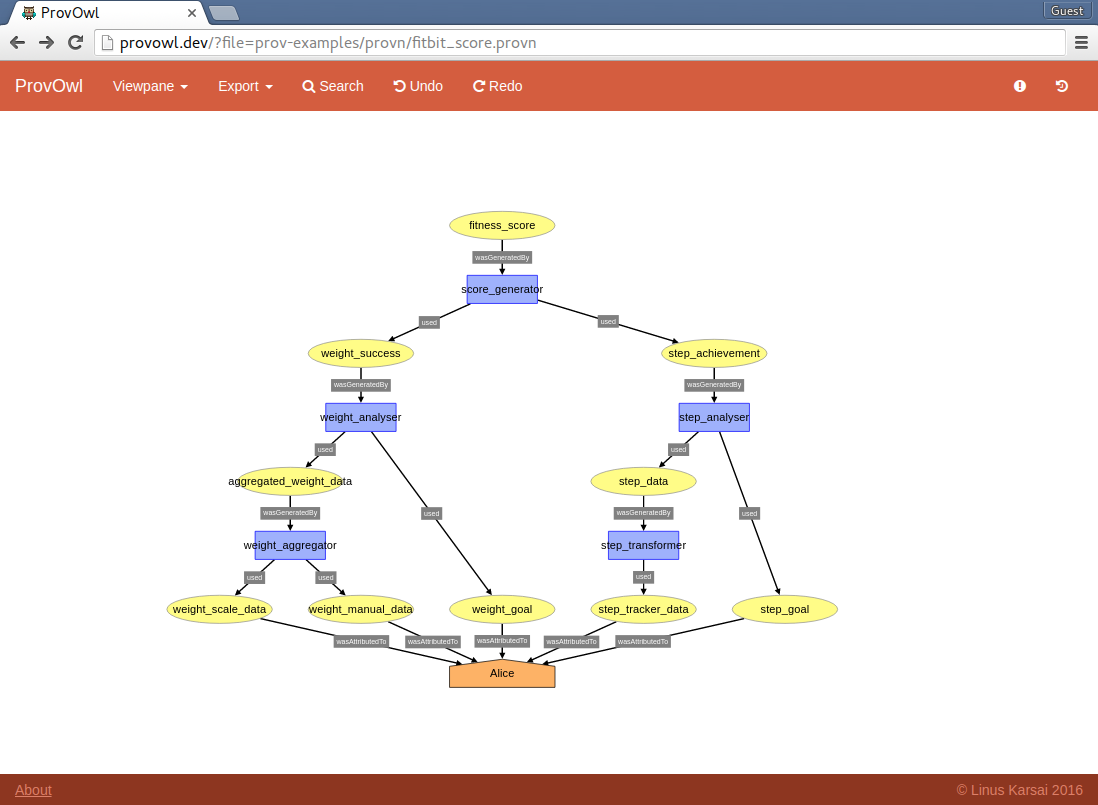
\includegraphics[width=\linewidth]{interface-example}
\caption{A screenshot of ProvOwl rendering the \texttt{fitbit\_score} prov file used in the usability studies.}
\label{fig:interface-example}
\end{figure}

When designing and selecting the features I would implement I used Ben Shneiderman's paper \textit{The eyes have it}~\cite{Shneiderman1996} as a foundation. In this paper he outlines seven visualisation tasks that are a useful starting point for designing advance graphical user interfaces. The tasks (taken directly from Shneiderman's paper) are as follows:

\begin{itemize}
\item Overview: Gain an overview of the entire collection. 
\item Zoom : Zoom in on items of interest 
\item Filter: Filter out uninteresting items. 
\item Details-on-demand: Select an item or group and get details when needed.
\item Relate: View relations hips among items. 
\item History: Keep a history of actions to support undo, replay, and progressive refinement.
\item Extract: Allow extraction of sub-collections and of the query parameters. 
\end{itemize}

Whilst implementing ProvOwl I continually came back to this list of tasks as a grounding point. Below I describe the main features of the interface. 

\section{Movement and Rearranging}
\label{sec:movement_and_rearranging}

On first opening a provenance graph, the viewport is positioned to fit an entire graph on screen as seen in Figure~\ref{fig:interface-example}. This acomplishes the \textit{overview} task from above and allows the user to view all the provenance at once. Users can then pan around by clicking and dragging. Zooming is accomplished by pressing ctrl+[+,-] or by using the scroll wheel. In large graphs this allows users to zoom in on areas of interest. 

By default the graph's overall layout is detemined using a JavaScript library called dagre that generates layouts for directed acyclic graphs client side. The main skeleton of the algorithm implemented to acomplish this comes from the paper ``A technique for Drawing Directed Graphs''~\cite{Gansner1993}. In early prototypes other layout options where made available such as circle and breadth-first, but this confused users and where later removed in favor of using dagre exclusively for layout.

\begin{wrapfigure}{r}{0.3\textwidth}
	\centering
	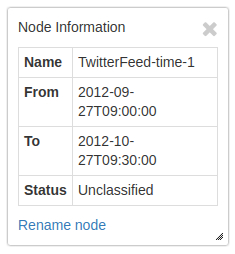
\includegraphics[width=\linewidth]{interface-details-close}
	\caption{A close up of the details panel from Figure~\ref{fig:interface-details}}
	\label{fig:key-concepts}
\end{wrapfigure}

Although initial placement is determined using the dagre algorithm, users can also re-arrange nodes manually by clicking and dragging a node. Note that this causes some issues when users are trying to pan, instead of cliking and dragging the background they accidentally click and move a node instead.

\section{Details on demand}
\label{sec:details_on_demand}

When a user selects a single or group of nodes the details panel is shown, as in Figure~\ref{fig:interface-details}. This displays information about the node as well as all its properties. At the bottom of the panel in blue text are contexual hyperlinks that enable functions such as renaming and in the case of multiple selected nodes, grouping. As suggested by the title, this directly immplements the taks of details-on-demand.

\begin{figure}[h]
	\centering
	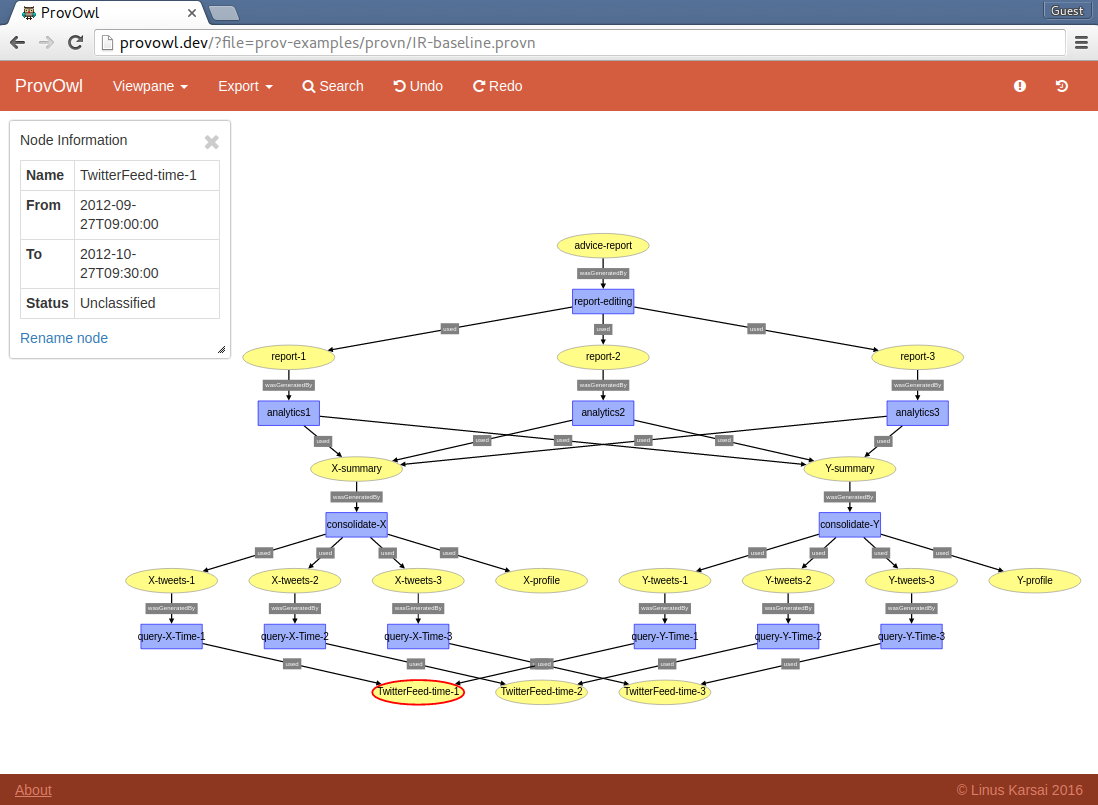
\includegraphics[width=\linewidth]{interface-details}
	\caption{A screenshot of ProvOwl with the \texttt{IR-baseline} prov file open. A indicated by the red outline, the node \texttt{TwitterFeed-time-1} has been selected and details about it such as name and classification status are shown in the details panel in the top left.}
	\label{fig:interface-details}
\end{figure}

\section{Clustering}
\label{sec:clustering}

As mentioned in Section~\ref{sec:user_defined_clusters} I have implemented two ways of clustering nodes, manually and via a search function. In both cases once the user activates the group function, the currently selected nodes are animated to their new position (the node closest to root) and replaced by a composite node, represented by a light blue oval. 

To manually cluster nodes a user first selects multiple nodes at once, by clicking on each whilst holding down \textit{ctrl}. Once multiple nodes have been selected the user cn group them together either with \textit{ctrl+g} or by selecting the group nodes hyperlink from the details panel.

The above method is tedious for more than a handful of nodes so I also implemented the search function. By opening up the search panel the user has access to a search field. The search function takes the value inputted by the user and runs a regex match on each property of each node. If any property of a node matches the regex it is selected (as indicated by a red outline).

In Figure~\ref{fig:search1} you can see an example of this. Open inside the ProvOwl interface is \textit{IR-baseline.prov}, an abstract example that shows the provenance of a report that is created to show analytical information about twitter data from two different users. On the right hand side of the screen is the search panel with the regex text \texttt{X-tweets|query-X-Time}. This query is run on all the nodes and because the pipe (\texttt{|}) characted represents an OR operator in regex hilights all the nodes that are either names \texttt{X-tweets-*} or \texttt{query-X-Time-*}. Once thses nodes are hilighted (as indicated by the red outline) they can be clustered into a composite node as seen in Figure~\ref{fig:search2}.


\begin{figure}[h]
	\centering
	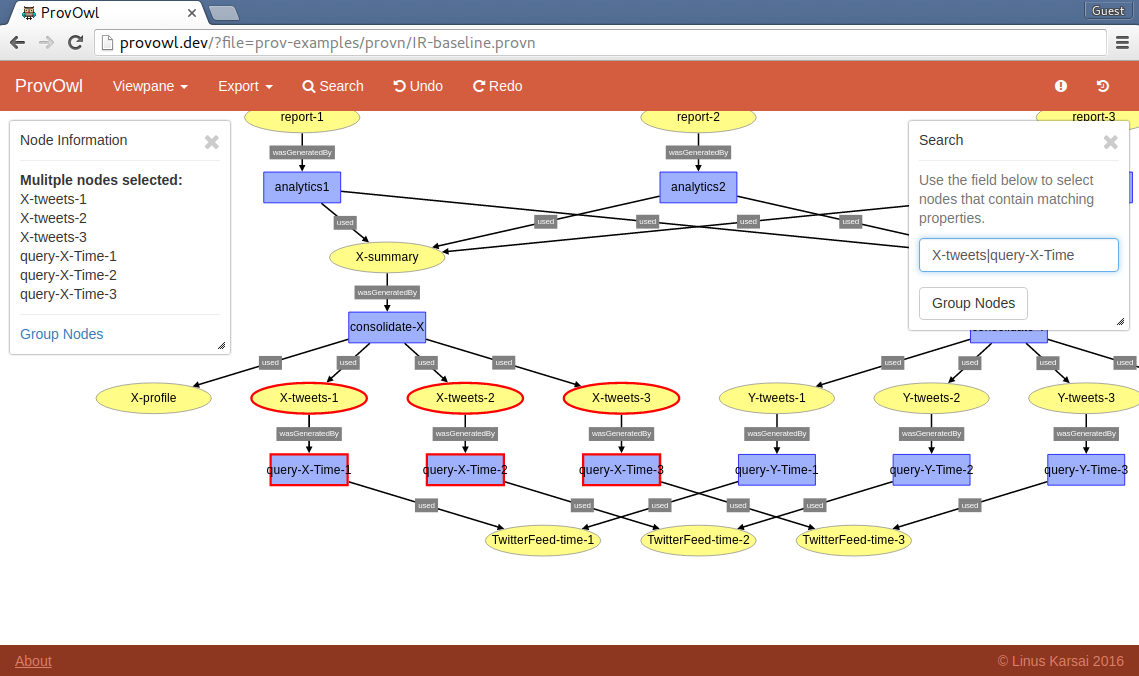
\includegraphics[width=\linewidth]{search1}
	\caption{A screenshot or ProvOwl with the \textit{IR-baseline.prov} file open; an abstract example that shows the provenance of an advice report presenting analytical information about twitter feeds. The search panel has been used to select a subset of the nodes.}
	\label{fig:search1}
\end{figure}
\begin{figure}[h]
	\centering
	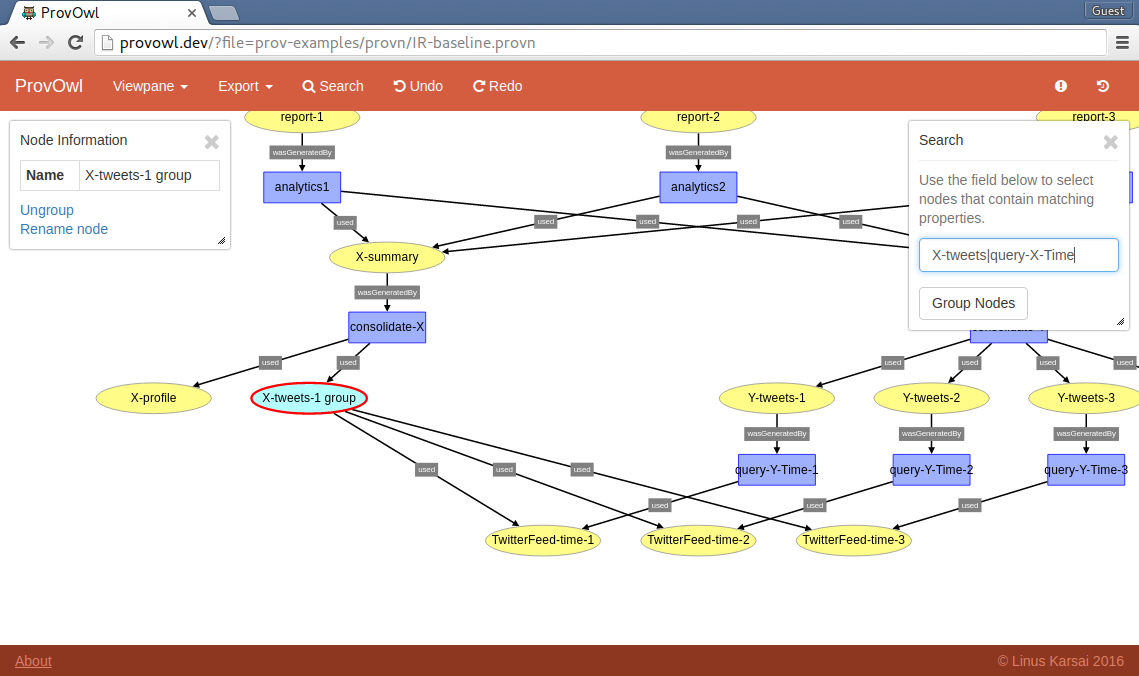
\includegraphics[width=\linewidth]{search2}
	\caption{Using the \textit{Group Nodes} button in the search panel, the nodes highlighted in Figure~\ref{fig:search1} have been clustered into a single composite node labelled \texttt{X-tweets-1 group}.}
	\label{fig:search2}
\end{figure}

\clearpage

\section{History}
\label{sec:history}

Having the ability to undo and redo actions is one of the above mentioned tasks for designing advance graphical interfaces and I believe one of the most important. It allows users to confidently and safely explore information without fear of causing permanent damage. My interface tracks primarily the movement and clustering of nodes. The undo and redo buttons allow users to step backwards and forwards through these actions. Using the history icon in the top right corner of the interface toggles a history pane (as seen in Figure~\ref{fig:interface-history}) that shows the user what step they are currently at. 

\begin{figure}[h]
	\centering
	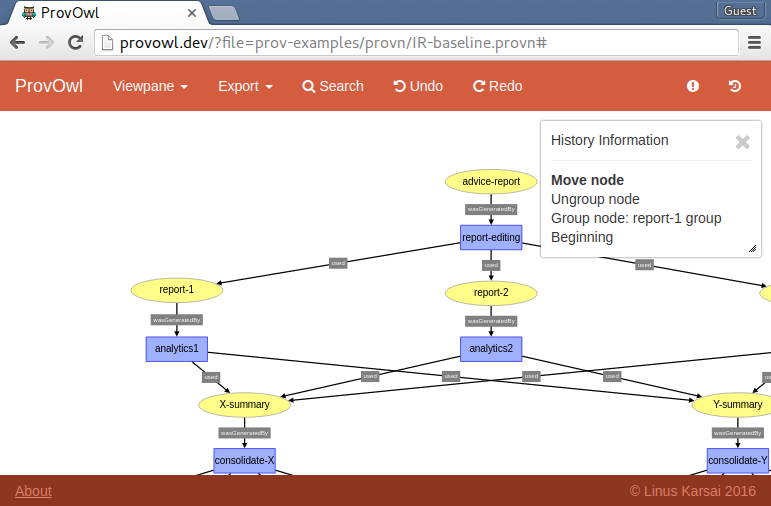
\includegraphics[width=0.8\linewidth]{interface-history}
	\caption{In the top right of the interface can be seen the history panel. This indicates what step of history the user is currently at. The user can use the undo and redo commands in the top bar to move backwards and forwards.}
	\label{fig:interface-history}
\end{figure}

\section{Sharing}
\label{sec:sharing}

In the top bar of Figure~\ref{fig:interface-history} there is a menu-bar option to export the current graph. This dropdown menu allows the user to either save the entire graph, or just the current viewport, as an image. The option to export just the viewport allows a user to focus on a certain section. This is related to the share task above and allows easy sharing of provenance files with other people for feedback and analysis. In the future I would also like to be able to export the current graph in PROV format with notation for clustered nodes.

\section{Click tracker}
\label{sec:click_tracker}

To facilitate with usability testing and by recommendation of Judy Kay I implemented a click tracker into the application. This simply logs clicks that the user makes, capturing time, location and element that the user clicked on. This could then be downloaded via the export command as a CSV file.  You can see below an example of the file generated from exploring the IR-baseline prov file.


\begin{figure}[h]
	\centering
	\lstinputlisting[style=basic]{misc/clickfile.csv}
	\caption{The CSV file generated from a user exploring the IR-baseline provenance file. Each line represent a single click by the user, a small description of the action they completed, what element it effected and the X,Y position of the click (if appropriate).}
	\label{fig:clickfile}
\end{figure}
